\documentclass[]{beamer}

\usepackage[T1]{fontenc}
\usepackage[brazilian]{babel}
\usepackage[utf8]{inputenc}

\usepackage{booktabs}
\usepackage{algorithm}
\usepackage{algorithmic}
\usepackage{subfig}
\usepackage{epstopdf}

\makeatletter
\newcommand{\newalgname}[1]{%
  \renewcommand{\ALG@name}{#1}%
}

\newalgname{Algoritmo}%
\usepackage{mdwlist}

\usetheme{CambridgeUS}
\usecolortheme[named=green]{structure}


\title[Analise de um dataset]
      {Analisando um \textit{dataset}: Acidentes em POA}

\date{Novembro de 2015}

% Author information
\author{$Gustavo\, J.\ Feller$; $William\, Lopes$}
\institute{INF/EA}

\AtBeginSection[]{
  \begin{frame}
  \vfill
  \centering
  \begin{beamercolorbox}[sep=8pt,center,shadow=true,rounded=true]{title}
    \usebeamerfont{title}\insertsectionhead\par%
  \end{beamercolorbox}
  \vfill
  \end{frame}
}

\begin{document}

% Command to create title page
\titlepage


\frame{
\begin{tiny}
  \tableofcontents
\end{tiny}
}

\section{Objetivo de negócio}
\frame{
\frametitle{Objetivo de negócio}
	\begin{itemize}
		\item Posicionar-se como gestor na área de trânsito na cidade de Porto Alegre
		\item Através de técnicas de Descoberta de Conhecimento em Base de Dados extrair informações para auxiliar na gestão do trânsito
		\item Utilizar a decisão baseada em fatos para recomendar modificações ou açõ
		\item Buscar a melhoria na segurança do trânsito em Porto Alegre
		\item Analisar observações de comportamento de acidentes de trânsito para evitar futuros acidentes
		\item Com os resultados aplicar modificações no trânsito (Sinalização, conscientização, intervenção, etc...)
	\end{itemize}
}

\section{Objetivo de mineração}
\frame{
\frametitle{Objetivo de mineração}
	\begin{itemize}
		\item Compreender a situação dos acidentes de trânsito na cidade de Porto Alegre
		\item Fornecer uma base para a tomada de decisões do objetivo de negócio
		\item Evidenciar informações relevantes para auxiliar na tomada de decisão
	\end{itemize}
}

\section{Dataset escolhido}
\frame{
\frametitle{\textit{Dataset} escolhido}
\begin{itemize}
	\item A base de dados escolhida foi o \textit{dataset} fornecido pelo governo municipal em relação aos acidentes de trânsito registrados em Porto Alegre
	\item A base escolhida conta com 14 \textit{datasets} sendo que cada \textit{dataset} representa um ano de registros, compreendendo o período de 2000 a 2014.
	\item Os dados são públicos e estão disponíveis para consulta juntamente com vários conjuntos de \textit{datasets} de outros setores do governo.
	\item Outros dois datasets com a localização dos pardais e a localização das lombadas eletrônicas foram utilizados.
\end{itemize}
}

\frame{
\frametitle{\textit{Dataset} escolhido}
\begin{table}[h]
	\begin{tiny}
	\begin{center}
	\caption{Estrutura do \textit{dataset}} \label{tab:dataset1}
	\begin{tabular}{|p{1.3cm}|p{3.5cm}|p{0,2cm}|p{1.3cm}|p{3.5cm}|} 
\cline{1-2} \cline{4-5} \multicolumn{1}{|c|}{\textbf{Campo}} & \multicolumn{1}{c|}{\textbf{Descritivo}} & & \multicolumn{1}{c|}{\textbf{Campo}} & \multicolumn{1}{c|}{\textbf{Descritivo}} \\ \cline{1-2} \cline{4-5}
Id          & Sequencial                     && Moto        & Motos envolvidas                    \\ \cline{1-2} \cline{4-5}
Log1        & Logradouro                     && Carroca     & Carroças envolvidas                 \\ \cline{1-2} \cline{4-5}
Log2        & Logradouro 2                   && Bicicleta   & Bicicletas envolvidas               \\ \cline{1-2} \cline{4-5}
Predial1    & Número próximo                 && Outro       & Outros veículos envolvidos          \\ \cline{1-2} \cline{4-5}
Local       & Tipo de logradouro             && Tempo       & Cond. Meteorológica                 \\ \cline{1-2} \cline{4-5}
Tipo\_Acid  & Tipo de acidente               && Noite\_Dia  & Momento do acidente                 \\ \cline{1-2} \cline{4-5}
Local\_Via  & Endereço acidente              && Fonte       & Fonte da ocorrencia                 \\ \cline{1-2} \cline{4-5}
Data\_hora  & Data e hora do ac.             && Boletim     & Num. Boletim ocorrencia             \\ \cline{1-2} \cline{4-5}
Dia\_sem    & Dia da semana                  && Regiao      & Região da cidade                    \\ \cline{1-2} \cline{4-5}
Feridos     & Num. feridos                   && Dia         & Dia do acidente                     \\ \cline{1-2} \cline{4-5}
Morte       & Num. Mortes                    && Mes         & Mês do acidente                     \\ \cline{1-2} \cline{4-5}
Morte\_post & Num. Mortes posterior          && Ano         & Ano do acidente                     \\ \cline{1-2} \cline{4-5}
Fatais      & Acidentes fatais               && Fx\_hora    & Faixa de hora do acidente           \\ \cline{1-2} \cline{4-5}
Auto        & Automóveis envolvidos          && Cont\_acid  & Núm. de carros envolvidos           \\ \cline{1-2} \cline{4-5}
Taxi        & Taxis envolvidos               && Cont\_Vit   & Núm. de vítimas no momento          \\ \cline{1-2} \cline{4-5}
Lotacao     & Lotações envolvidas            && UPS         & Núm. de atendidos por UPS           \\ \cline{1-2} \cline{4-5}
Onibus\_urb & Ônibus urb. envolvidos         && Latitude    & Latitude                            \\ \cline{1-2} \cline{4-5}
Onibus\_int & Ônibus int. envolvidos         && Longitude   & Longitude                           \\ \cline{1-2} \cline{4-5}
Caminhão    & Caminhões envolvidos           &\multicolumn{1}{c}{}& \multicolumn{1}{c}{}& \multicolumn{1}{c}{}        \\ \cline{1-2}
		\end{tabular} 
	\end{center}
	\end{tiny}
\end{table}
}

\section{Pré-processamento}
\frame{
\frametitle{Pré-processamento}
\begin{itemize}
	\item Retirada de campos não considerados:
	\begin{itemize}
		\item \textbf{Id:} Sequencial do arquivo, considerado como não relevante, visto informações de data e hora do acidente.
		\item \textbf{Boletim:} Boletim de ocorrência, sequencial sem relação com outros campos.
		\item \textbf{Data\_Hora:} Data e hora do acidente, campo duplicado, considerado que o campo "FX\_hora"\ é mais relevante para classificação.
		\item \textbf{Data:} Duplicado de "Data\_Hora"\ e campos "Dia", "Mes"\ e "Ano"\ contém as informações a um nível mais detalhado
		\item \textbf{Fonte:} O campo fonte do registro do acidente não se enquadrou nos objetivos do presente trabalho
	\end{itemize}
\end{itemize}
}

\frame{
\frametitle{Pré-processamento}
\begin{itemize}
	\item Análise de campos vazios (Ex: Log2 , Hora $<1\%$) - Linhas com colunas relevantes que estavam vazias foram retiradas (3 linhas no total)
	\item Coluna de fatalidade (S para sim ou N para não), existe a coluna com quantidade de fatalidades e de mortes pós acidente.
	\item Criação de um dataset auxiliar apenas com as linhas ao qual houveram acidentes fatais (LOG1, LOCAL, TIPO ACID, DIA SEM, TEMPO, NOITE DIA e REGIAO).
	\item Datasets auxiliares (lombadas e pardais) foram designados latitude e longitude pois tinham apenas uma coluna, o endereço, sendo retirado dados duplicados.
	\item Ajustes necessários em latitude e longitude, mesmo sendo um dataset preparado para kdd
\end{itemize}
}

\section{Mineração de dados}
\frame{
\frametitle{Mineração de dados - Análise dos dados}
\begin{itemize}
	\item Analisados os últimos 4 anos, sendo que foram trabalhados:
	\begin{itemize}
		\item Histogramas para conhecimento da estrutura (horários acidentes, dias acidentes, meses acidentes)
		\item "Ranges" por dataset
		\item Algoritmo \textit{apriori} em características de acidentes fatais
		\item Tentativa de k-nn
		\item Visualização de densidade de acidentes (\textit{heatmap}) em mapa (latitude/longitude) com localização de lombadas e pardais
	\end{itemize}
\end{itemize}
}

\frame{
\frametitle{Mineração de dados - Análise dos dados}
\begin{table}[h]
	\begin{center}
		\begin{tiny}
		\caption{Número de acidentes por ano e número de acidentes fatais por ano} \label{tab:dataset}
		\begin{tabular}{r|r|r|r|r|r|r|r}
		\hline
\multicolumn{1}{c|}{\textbf{Ano}} & \multicolumn{1}{c|}{\textbf{Acid.}} & \textbf{Fatais} & \textbf{\% Fatais} & \multicolumn{1}{c|}{\textbf{$\dagger$}} & \multicolumn{1}{c|}{\textbf{Máx. $\dagger$}} & \multicolumn{1}{c|}{\textbf{Máx. $\dagger$ pós}} & \multicolumn{1}{c}{\textbf{Máx tot. $\dagger$}} \\ \hline
2011 & 23.579 & 135 & $0,57$ & 141 & 3 & 2 & 3 \\
2012 & 20.202 & 97  & $0,48$ & 100 & 1 & 2 & 2 \\
2013 & 20.799 & 117 & $0,56$ & 124 & 4 & 1 & 5 \\
2014 & 17.203 & 135 & $0,78$ & 135 & 1 & 1 & 1 \\ \hline
\multicolumn{1}{l|}{\textbf{Total}} & 81.703 & 484 & $0,59$ & 500 & - & - & - \\ \hline
		\end{tabular}
		\end{tiny}
	\end{center}
\end{table}
}


\frame{
\frametitle{Mineração de dados - Histogramas}
\begin{figure}[h!]
	\caption{Histogramas dos horários dos acidentes entre 2011 e 2014} \label{fig:histhora}
    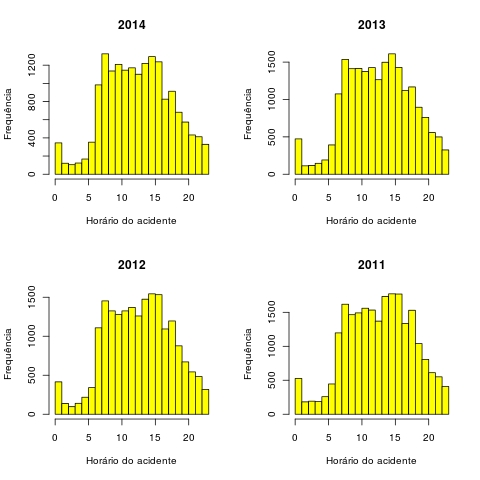
\includegraphics[width=.5\textwidth]{horas_acidentes.jpg}
\end{figure}
}

\frame{
\frametitle{Mineração de dados - Correlação}

\begin{table}[h]
	\begin{center}
		\begin{tiny}
		\caption{Correlação entre acidentes com tipo de condução em 2014} \label{tab:corr}
		\begin{tabular}{l|r|r|r|r|r|r|r|r|r|r|r} \hline
\multicolumn{1}{c|}{\textbf{Tipo}}& \multicolumn{1}{c|}{\textbf{Auto}}& \multicolumn{1}{c|}{\textbf{Taxi}} & \multicolumn{1}{c|}{\textbf{Lot.}} & \multicolumn{1}{c|}{\textbf{O.U.}} & \multicolumn{1}{c|}{\textbf{O.M.}} & \multicolumn{1}{c|}{\textbf{O.I.}} & \multicolumn{1}{c|}{\textbf{Cam.}} & \multicolumn{1}{c|}{\textbf{Mot.}} & \multicolumn{1}{c|}{\textbf{Car.}} & \multicolumn{1}{c|}{\textbf{Bic.}} & \multicolumn{1}{c}{\textbf{Out.}} \\ \hline
$\dagger$  & -0.054 & -0.018 & -0.001 & 0.022 & 0.011 & 0.003 & 0.018 & 0.025 & -0.001 & 0.037 & -0.003 \\
F.G. & -0.163 & -0.031 & -0.017 & 0.005 & 0.010 & -0.004 & -0.038 & 0.187 & 0.014 & 0.024 & 0.001 \\
		\hline
		\end{tabular}
		\end{tiny}
	\end{center}
\end{table}
}

\frame{
\frametitle{Algoritmo \textit{apriori}}
\begin{itemize}
	\item Aplicado ao dataset completo, sem relevância para acidentes do tipo fatal
	\item Dataset auxiliar apenas com os acidentes fatais foi utilizado
	\begin{itemize}
		\item Atropelamentos ocorrem principalmente no centro e de dia
		\item Av. Baltazar de Oliveira Garcia tem forte relação com acidentes fatais à noite
	\end{itemize}
\end{itemize}
}

\frame{
\frametitle{Mineração dos dados - Densidade de acidentes}
\begin{itemize}
	\item Adicionado densidade ao mapa por tipo de acidente, pela latitude e longitude
	\item Interatividade via Google Maps
	\item Utilizado os datasets das lombadas eletronicas e pardais
\end{itemize}
}

\frame{
\frametitle{Mineração dos dados - Densidade de acidentes}
\begin{figure}[h!]
	\caption{Heatmap com os acidentes no ano de 2014} \label{fig:densgeral}
    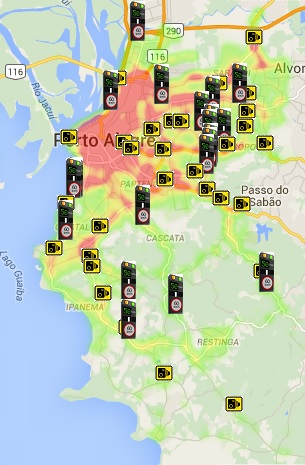
\includegraphics[width=.3\textwidth]{densidade_geral_2014.jpg}
\end{figure}
}

\frame{
\frametitle{Mineração dos dados - Densidade de acidentes}
\begin{figure}[h!]
	\caption{Heatmap com os acidentes fatais no ano de 2014} \label{fig:densfatal}
    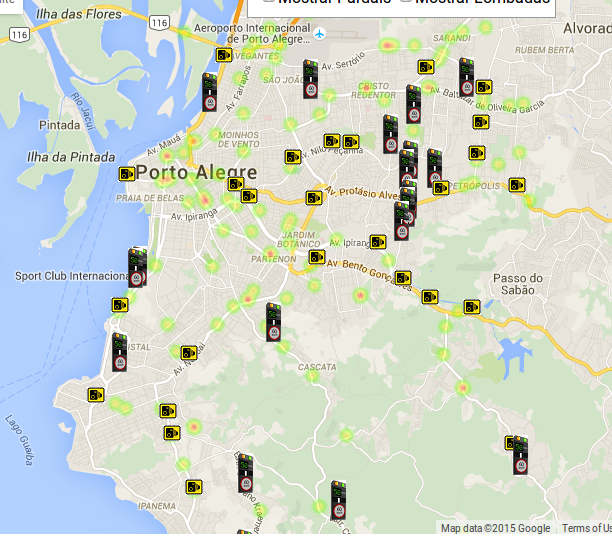
\includegraphics[width=.5\textwidth]{densidade_acidentes_2014.jpg}
\end{figure}
}

\frame{
\frametitle{Conclusões}
\begin{itemize}
	\item Os histogramas de densidade no horário de acidente inicia-se às 6 horas da manhã e tem seu pico às 3 horas da tarde, diminuindo consideravelmente após esse horário.
	\item Também, o mapa com a densidade dos acidentes comprovou que locais com controladores de velocidade e pardais os acidentes fatais são bem raros, mostrando-se um sistema eficiente para diminuição dos acidentes. Outro ponto importante que pode ser visto no mapa são os locais com maiores quantidades de acidentes. 
	\item Também notou-se que os acidentes mais graves ocorrem em entradas de vias principais, como, por exemplo, a Av. Bento Gonçalves. Nas próprias avenidas não há registros de acidentes graves, porém, logo após as entradas secundárias destas avenidas pode-se verificar registros com densidades consideráveis de serem avaliadas.
\end{itemize}
}

\frame{
\frametitle{Sugestões}
\begin{itemize}
	\item[-] Melhorar sinalização nas esquinas, principalmente nas vias de entrada das principais avenidas por conterem o maior número de acidentes do tipo fatais (no heatmap fica claro).
	\item[-] Em vias com um grande número de acidentes fatais diminuir a velocidade máxima, como, por exemplo, a Estrada João de Oliveira Remião.
	\item[-] Aumentar a sinalização onde as densidades dos acidentes ocorrem mais
	\item[-] Refazer o KDD anualmente, na medida que as informações dos datasets estão disponíveis para verificar o comportamento do trânsito e inferir novas ações;
	\item[-] Sugestão de estudos futuros: \textit{Dataset} de blitz X acidentes fatais à noite.
\end{itemize}
}

\frame{
    \frametitle{Obrigado!}
    \parbox{\textwidth}{%
        \centering
        {\bfseries \insertauthor}~\\
        {\small \insertinstitute}~\\
        \vspace{30pt}
    }
}

%\titlepage

\end{document}
